\documentclass[conference]{IEEEtran}
\IEEEoverridecommandlockouts

\usepackage[T1]{fontenc}
\usepackage[utf8]{inputenc}
\usepackage{cite}
\usepackage{amsmath,amssymb}
\usepackage{graphicx}
\usepackage{booktabs}
\usepackage{array}
\usepackage{url}
\usepackage{hyperref}
% microtype removed (conflicts with IEEEtran)

\graphicspath{{../../plots/cv}}

\begin{document}

% --- Title -------------------------------------------------------------------
\title{Single-Shot Cup Aim Prediction for a 3-axis Ping Pong Ball Launcher}

\author{
  \IEEEauthorblockN{Ryan Schmidt\thanks{Code available at: \url{https://github.com/rschmi3/pong-bot}}}
  \IEEEauthorblockA{
    Department of Computer Science\\
    Western University\\
    rschmi3@uwo.ca
  }
}

\maketitle

% --- Abstract ----------------------------------------------------------------
\begin{abstract}
This paper presents an end-to-end computer vision pipeline for predicting
continuous motor step values to aim a ping-pong ball launcher at a cup, using
a single camera image on a Raspberry Pi. A custom PongDetector CNN (1.52\,M
parameters) detects the cup, followed by an aim head that maps visual features
and bounding box geometry to motor step targets derived from noisy
reinforcement learning pseudo-labels. A key finding is that backbone features
explain only $r^{2}=0.117$ of horizontal motor position variance, while
bounding box centre-$x$ achieves $r^{2}=0.981$, motivating explicit bounding
box concatenation. Three aim head architectures were developed iteratively; the
final split-head design (V3) achieves a 33\% live hit rate across 24 of 30 cup
positions. A sim-to-live gap analysis is introduced as a deployment reliability
metric. Future work includes improved camera geometry, additional depth features,
arbitrary cup placement, and multi-cup detection for sequential shot planning.
\end{abstract}

% --- I. Introduction ---------------------------------------------------------
\section{Introduction}

Autonomous physical robots that interact with the real world via vision face a
fundamental challenge: translating raw pixel data into actionable control
signals. This paper addresses a concrete instance of that challenge in the
Pong-Bot project, a tabletop robot that launches ping-pong balls at a small cup
placed anywhere on a 6-foot table. A fixed camera is mounted on the base of the
launcher, and the robot has no depth sensor and no map of the environment.
Given a single $640{\times}640$ RGB image, the system must predict the two
motor step values ($x_\text{steps}$, $y_\text{steps}$) required to aim the
launcher at the visible cup and hit it in a single shot.

The problem seems straightforward, but proves to be deceptively difficult.
First, depth must be inferred solely from apparent cup size in the image, since
the camera is mounted nearly level with the table surface, causing vertical
image position to vary by only 1.5\% across the full depth range. Second,
ground-truth aim labels must be collected experimentally, which is a time
consuming process. The training requires not only images with bounding box labels,
but also a ground truth mapping of bounding box to motor step values. In our case
images were gathered with a Reinforcement Learning (RL) pipeline, generating
noisy pseudo-labels from shot convergence. Third, inference must run on a
Raspberry Pi without PyTorch, requiring a float32-only ONNX export compatible
with OpenCV's \texttt{cv2.dnn} backend.

Prior work on robot aim prediction typically relies on depth
sensors~\cite{saxena2008,redmon2015} or 3-D pose estimation
pipelines~\cite{lepetit2009}.  No prior work has addressed direct motor step
regression from a single 2-D image under embedded deployment constraints
without depth information.  The contributions of this work are:
\begin{enumerate}
  \item An $r^{2}$ correlation analysis revealing that backbone features are
        position-blind ($r^{2}=0.117$ with $x$-position), motivating explicit
        bounding box concatenation in the aim head.
  \item Three iteratively designed aim head architectures (V1/V2/V3) achieving
        progressive improvement in live hit rate.
  \item A float32-only ONNX deployment pipeline for \texttt{cv2.dnn} on
        Raspberry Pi.
  \item Per-cell median pseudo-label denoising for noisy RL-derived training
        targets.
\end{enumerate}

The best model, V3 (split-head), achieves a 33\% live hit rate and covers 24
of 30 distinct cup positions, demonstrating that explicit geometric features
outperform learned representations for spatial regression in
resource-constrained robotics.

% --- II. Background ----------------------------------------------------------
\section{Background and Related Work}
\label{sec:background}

\subsection{Object Detection}

The YOLO family~\cite{redmon2016} introduced single-stage, anchor-based fully
convolutional detectors that predict class probabilities and bounding box
offsets on a regular grid.  PongDetector follows a similar design with an
$80{\times}80$ YOLO-style grid head, adapted for single-class detection on a
small embedded device.  Subsequent versions (YOLOv5~\cite{jocher2020},
YOLOv8~\cite{jocher2023}) scaled this approach with larger, more complex
architectures optimised for multi-class detection across diverse scenes; this
capacity is unnecessary for a single-class, single-object detection task,
motivating a lightweight from-scratch design.

\subsection{Architecture Components}

He et al.~\cite{he2016} showed that residual connections enable training of
very deep networks with strong generalisation.  PongDetector's encoder uses
ResNet-style residual blocks.  Squeeze-and-Excitation (SE)
networks~\cite{hu2018} introduced channel attention, recalibrating feature
responses to emphasise informative channels; each ResConvBlock in PongDetector
incorporates an SE module.  In the aim head training phase the backbone is
frozen and only the aim head is updated, preventing catastrophic forgetting of
detection features.

\subsection{Research Gap}

Prior work on vision-based robot aiming and
grasping~\cite{redmon2015,levine2018} relies on depth sensors, stereo rigs, or
large robot fleets for data collection.  Our RL-derived motor targets are a form
of weak pseudo-labelling: the winning motor position found by RL after many
shots serves as a noisy proxy for the true optimal aim.  Median aggregation
across noisy labels reduces label variance; we apply this principle through
per-cell median $Y$-target denoising.  No prior work combines single-object
detection with direct continuous motor step regression from noisy RL-derived
pseudo-labels under embedded deployment constraints.  This work fills that gap.

% --- III. Dataset ------------------------------------------------------------
\section{Dataset and Pseudo-Labels}
\label{sec:dataset}

\subsection{Roboflow Labelling Pipeline}

Images were captured during RL data-collection sessions in which the robot
fired at the table while the camera was mounted on the launcher.  Each image
was manually annotated in Roboflow with a tight bounding box around the cup.
Labels are stored in YOLO format (\texttt{class\_id cx cy w h}), normalised to
$[0,1]$.  The dataset was split into training, validation, and test subsets and
retrieved via the Roboflow Python SDK.  Table~\ref{tab:splits} summarises the
split statistics.

\begin{table}[ht]
\centering
\caption{Dataset Split Statistics}
\label{tab:splits}
\begin{tabular}{lrrr}
\toprule
Split & Total & Positive & Negative \\
\midrule
Train & 913  & 833  & 80  \\
Valid & 233  & 223  & 10  \\
Test  & 121  & 111  & 10  \\
\midrule
\textbf{Total} & \textbf{1267} & \textbf{1167} & \textbf{100} \\
\bottomrule
\end{tabular}
\end{table}

\subsection{Aim Head Training Data and Pseudo-Labels}

Each shot record in \texttt{shots.jsonl} links a camera image to the motor
position at fire time.  The ground-truth aim target is not the fired position
but the \emph{winning position} from the RL session; the motor position that
eventually produced a hit.  Because RL convergence introduces noise, two
denoising strategies are applied.

\textbf{Gaussian distance weighting.}  Every shot that belongs to a session
that converged to a hit contributes to training with weight
$w = \exp(-d/T)$, where $d$ is the Euclidean distance in motor-step space from
the shot position to the winning position and $T=2000$ steps.  Direct hits
receive weight $1.0$; shots far from the winning position are down-weighted.

\textbf{Per-cell median $Y$ target.}  The winning $Y$ position varies between
RL sessions for the same cup location due to convergence noise.  The $Y$
training target uses the median winning $Y$ across all sessions that hit the
same (cup$_x$, cup$_y$) grid cell, reducing pseudo-label noise from
approximately 1000 steps to 300-500 steps per cell.

% --- IV.  Methods -------------------------------------------------------------
\section{Methods}
\label{sec:methods}

\subsection{Research Objectives}

Four objectives guided the system design: \textbf{(1)}~deploy a float32-only
ONNX detector on Raspberry Pi via \texttt{cv2.dnn} without PyTorch;
\textbf{(2)}~determine which visual signals best predict motor steps via $r^{2}$
correlation analysis; \textbf{(3)}~develop and compare iterative aim head
architectures (V1/V2/V3); \textbf{(4)}~evaluate the sim-to-live gap as a
deployment reliability metric.

\subsection{PongDetector Architecture}

PongDetector is a from-scratch CNN with 1.52\,M parameters.  The encoder
consists of four ResConvBlocks with Squeeze-and-Excitation channel attention
and residual connections, progressively downsampling from $640{\times}640$ to
$80{\times}80$ pixels while increasing channel depth from 3 to 256.  A fully
convolutional detection head with a $1{\times}1$ convolution produces a
5-channel output, centre offsets, width/height scaling, and a detection score,
on the $80{\times}80$ grid.  Grid decoding follows the YOLO convention: centre
coordinates are predicted as sigmoid offsets from the cell corner, and
width/height are log-scale corrections to automatically computed anchors (mean
ground-truth box dimensions from the training set).

The training loss combines CIoU bounding box loss~\cite{zheng2020} (weight
$=5.0$) with focal loss~\cite{lin2017} on the score channel ($\alpha=0.25$,
$\gamma=2.0$, positive weight $=100$).  Positive assignment uses a $3{\times}3$
cell neighbourhood around the ground-truth cell centre, which eliminates the
systematic prediction offset caused by single-cell assignment.  Data
augmentation includes horizontal flipping, random scale/crop, translation,
colour jitter, Gaussian noise, blur, and cutout.

For the aim head, two feature vectors are extracted from the best-scoring
detection cell: a local cell feature (the 256-dimensional encoder map at the
best cell) and a global feature (global average pooling of the full
$80{\times}80$ encoder map).  These are concatenated to form a 512-dimensional
feature vector passed to the aim head.

\begin{figure}[ht]
  \centering
  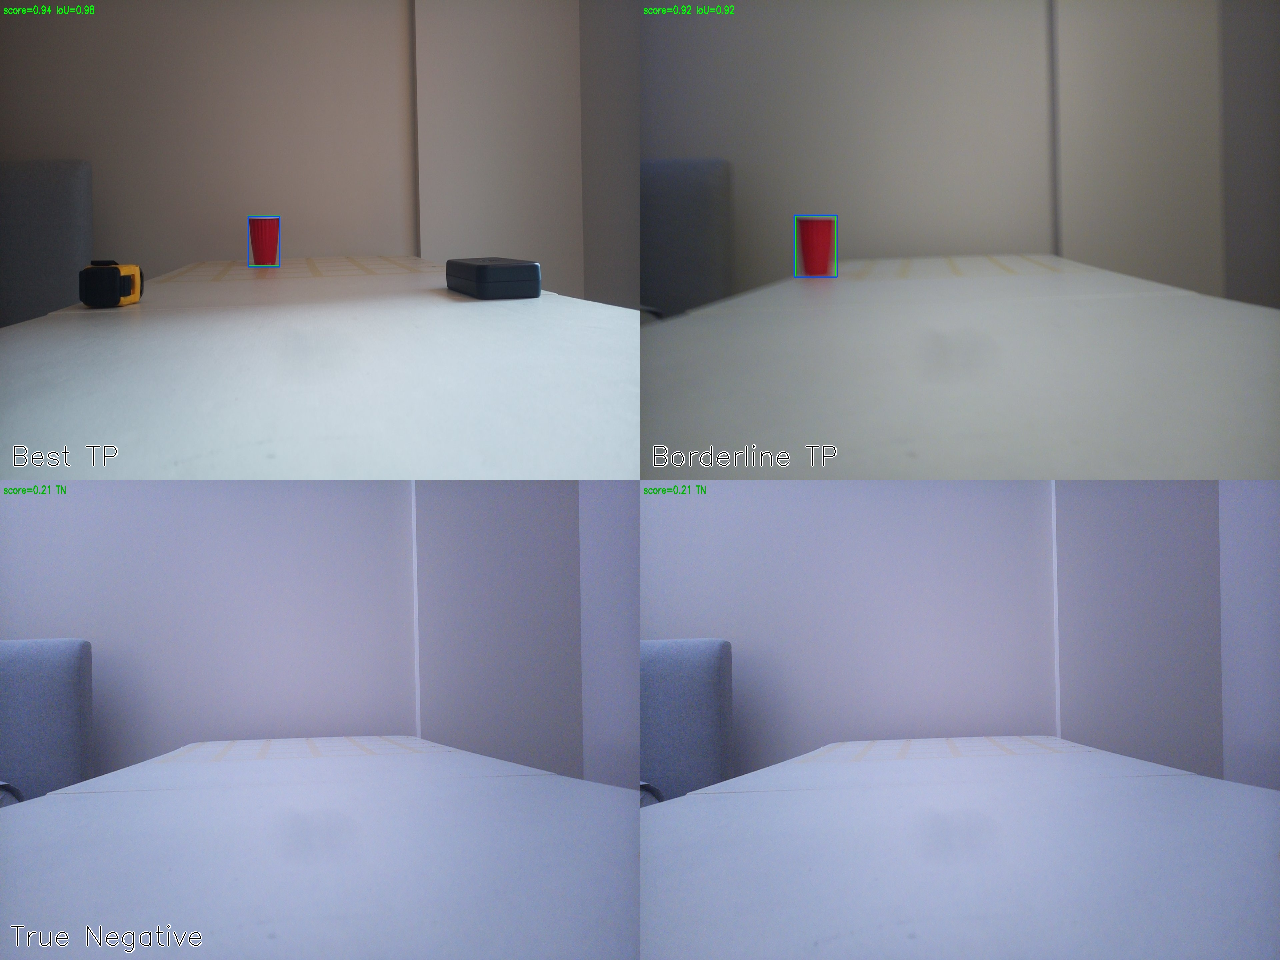
\includegraphics[width=\columnwidth]{cv_detect_grid.png}
  \caption{Detector test results on the held-out test set (111 positive,
  10 negative images). \textbf{Top row:} best true positive (IoU\,=\,0.981,
  score\,=\,0.941) and a borderline true positive (IoU\,=\,0.917,
  score\,=\,0.923). \textbf{Bottom row:} true negative images correctly
  rejected (score\,=\,0.21).  Green boxes are model predictions; blue boxes
  are ground-truth annotations.}
  \label{fig:detect}
\end{figure}

\subsection{Feature Analysis and Motivation for Bounding Box Concatenation (2)}

Before designing the aim head, an $r^{2}$ correlation analysis was performed on
1167 labelled shot images to determine which visual signals predict the motor
step targets.  The results appear in Fig.~\ref{fig:r2} and
Table~\ref{tab:r2}.

\begin{figure}[ht]
  \centering
  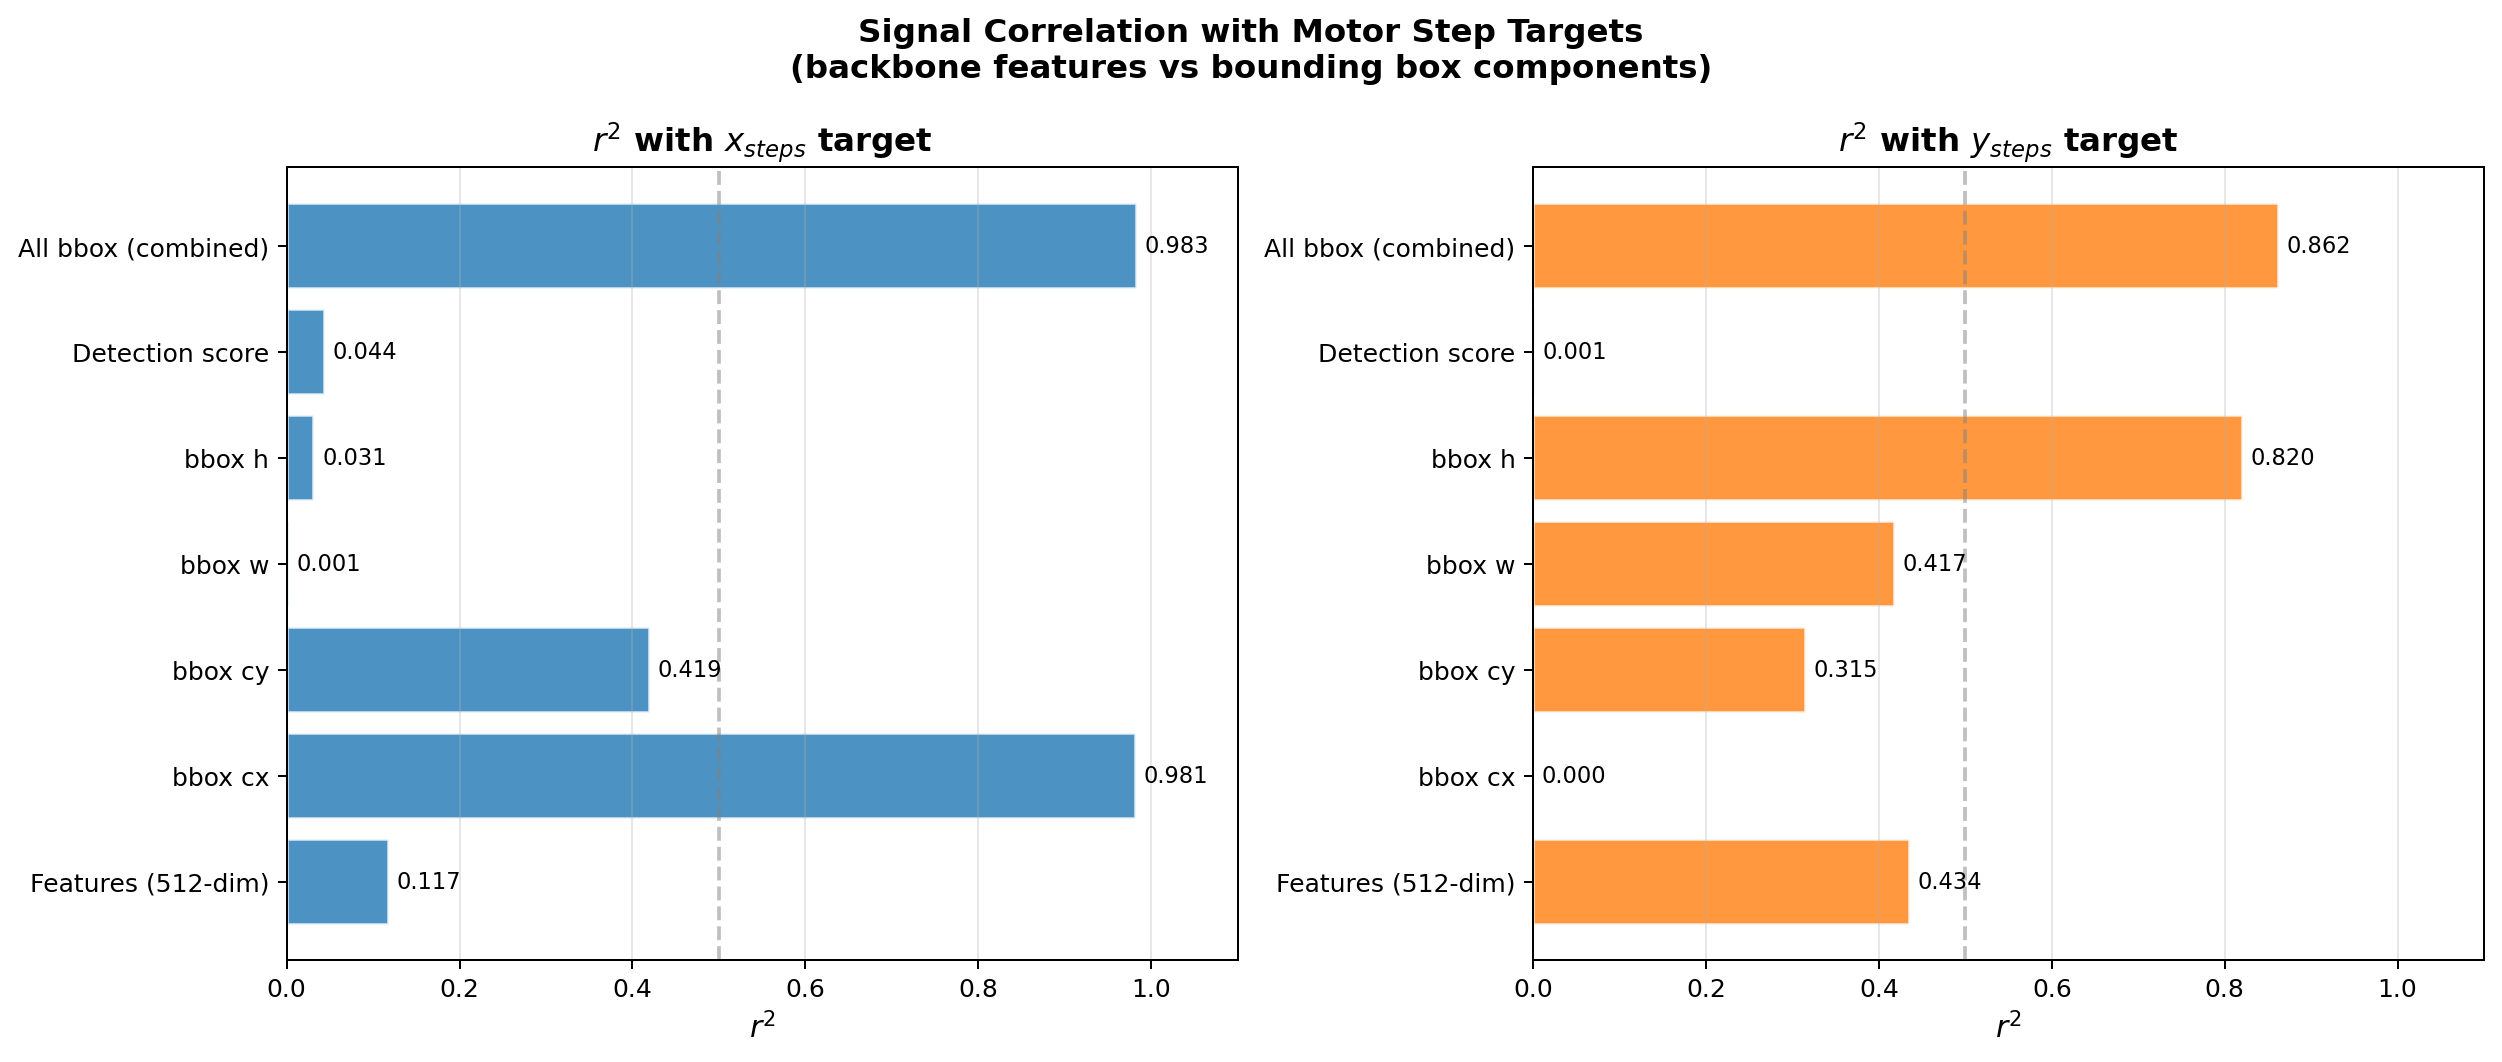
\includegraphics[width=\columnwidth]{cv_r2_analysis.png}
  \caption{$r^{2}$ correlation of individual visual signals with motor step
  targets $x_\text{steps}$ (blue, left panel) and $y_\text{steps}$ (orange,
  right panel).  Backbone features (512-dim, best linear direction) explain
  only $r^{2}=0.117$ of $x$-position variance, while \texttt{bbox cx}
  achieves $r^{2}=0.981$.  For $y$-position, \texttt{bbox h}
  ($r^{2}=0.820$) dominates, encoding cup distance through apparent cup
  height.}
  \label{fig:r2}
\end{figure}

\begin{table}[ht]
\centering
\caption{$r^{2}$ Correlation of Visual Signals vs.\ Motor Step Targets}
\label{tab:r2}
\begin{tabular}{lcc}
\toprule
Signal & $r^{2}$ with $x_\text{steps}$ & $r^{2}$ with $y_\text{steps}$ \\
\midrule
Backbone features (512-dim) & 0.117 & 0.434 \\
bbox $c_x$                  & \textbf{0.981} & 0.000 \\
bbox $c_y$                  & 0.419 & 0.315 \\
bbox $w$                    & 0.001 & 0.417 \\
bbox $h$                    & 0.031 & \textbf{0.820} \\
Detection score             & 0.044 & 0.001 \\
All bbox (multiple reg.)    & \textbf{0.983} & 0.862 \\
\bottomrule
\end{tabular}
\end{table}

The backbone is effectively position-blind: its best linear direction explains
only $r^{2}=0.117$ of $x$-position variance.  This is expected, as the
detection backbone learned features useful for recognising the cup, not for
encoding its absolute location in motor-step space.  In contrast, bbox $c_x$
alone achieves $r^{2}=0.981$, confirming a near-linear mapping from horizontal
image position to horizontal motor steps.  For the $Y$ axis, bbox $h$ achieves
$r^{2}=0.820$, encoding depth: a cup farther from the launcher appears smaller
in the image, requiring more elevation.  All four bbox components combined
achieve $r^{2}=0.983$ ($X$) and $r^{2}=0.862$ ($Y$) through linear regression
alone, establishing that the MLP aim head learns a small residual correction on
top of this linear baseline.

\subsection{Aim Head Architecture Evolution (3)}

Three aim head versions were developed iteratively, each addressing weaknesses
identified through live testing.

\textbf{V1 (516-dim, baseline)} concatenates the 512-dimensional backbone
features with raw bounding box coordinates $(c_x, c_y, w, h)$, producing a
516-dimensional input.  A two-hidden-layer MLP (256 and 128 units, ReLU
activations, 0.2 dropout) maps this to two output values, normalised to
$[-1,1]$ through Tanh and denormalised as $x_\text{steps}{\times}10\,000$ and
$y_\text{steps}{\times}20\,000$.

\textbf{V2 (518-dim)} adds two derived features: aspect ratio ($h/w$) and
box area ($w{\times}h$), motivated by live testing of V1 that revealed poor
$Y$-axis prediction.  Because the camera is mounted nearly level with the
table, cup vertical image position $c_y$ varies by only 1.5\% across the full
depth range, making it a weak depth cue.  Bounding box height $h$ varies by
40\%, providing the dominant depth signal.  Explicit aspect ratio and area
features amplify this signal.

\textbf{V3 (split heads)} uses separate $X$ and $Y$ prediction heads after
observing that V2's $Y$-oriented derived features interfered with $X$
prediction ($X$ accuracy regressed in V2).  The $X$ head receives features $+$
bbox $c_x$ (513 dimensions); the $Y$ head receives features $+$ bbox $h$ $+$
aspect $+$ area (515 dimensions).  Each head has a single hidden layer
(128 units) predicting one scalar.  V3 is also the most parameter-efficient
(132\,098 parameters vs.\ 165\,506 for V1) because each head predicts one
scalar rather than two.

\subsection{ONNX Deployment (1)}

The full model (detector + aim head) is exported to ONNX via
\texttt{torch.onnx.export} and loaded on the Raspberry Pi using
\texttt{cv2.dnn.readNetFromONNX}, eliminating the PyTorch dependency at
inference.  OpenCV's ONNX backend has limited operator coverage; PyTorch's
default dtype promotion and dynamic shape tracing silently introduced int64
and float64 graph nodes that the backend could not execute.  All anchor
buffers, grid coordinates, and index operations were rewritten as static
float32 equivalents to produce a compatible graph.

\subsection{Threats to Validity}

\textbf{Small live test set.}  The live evaluation totals 229 shots across
three models (68 + 66 + 95).  Per-model confidence intervals are wide;
differences of a few percentage points in hit rate should be interpreted
cautiously.

\textbf{Fixed experimental setup.}  All data were collected with a single
camera angle and table configuration.  Results may not generalise to different
mounting geometries or table surfaces.

\subsection{Rationale for Key Design Decisions}

\textbf{CIoU + focal loss over BCE.}  CIoU provides richer gradient signal for
small bounding boxes by incorporating aspect ratio and centre distance in
addition to overlap.  Focal loss addresses the severe class imbalance in the
$80{\times}80 = 6400$-cell grid where only 1-9 cells contain a cup.

\textbf{Frozen backbone for aim head training.}  Fine-tuning the backbone while
training the aim head risks catastrophic forgetting of the detection features.
An optional \texttt{--unfreeze-backbone} flag is provided for differential
learning-rate fine-tuning when desired.

\textbf{Huber loss for aim head.}  The noisy pseudo-labels produced by RL
convergence create outlier targets; Huber loss with $\delta=1.0$ (in
normalised space) clips the gradient for large deviations, improving
robustness.

% --- V. Results --------------------------------------------------------------
\section{Results}
\label{sec:results}

\subsection{Embedded Deployment (1)}

The full model was exported to ONNX and loaded on the Raspberry Pi 4 using
\texttt{cv2.dnn.readNetFromONNX}, with no PyTorch dependency at inference.
The float32-only ONNX export produces predictions identical to the PyTorch
model.  Inference on a single $640{\times}640$ RGB frame takes approximately
830\,ms on the ARM Cortex-A72 CPU, which is acceptable for a single-shot
pipeline where one image is captured and inferred per firing cycle.

\subsection{Detector Performance}

Table~\ref{tab:detector} reports detector performance on the held-out test set
at a score threshold of $0.5$.  The detector achieves perfect classification
(100\% true positive rate, 100\% true negative rate, zero false positives and
zero false negatives) with a mean IoU of 0.848 on positive images.  The mean
positive score (0.952) is well separated from the mean negative score (0.334),
indicating a robust decision margin.  These results should be interpreted in
the context of the training conditions: all images were captured from a fixed
camera position with a single cup type against a consistent background, making
the detection task substantially simpler than general-purpose object detection
benchmarks.  Visual inspection of representative detections is shown in
Fig.~\ref{fig:detect}.

\begin{table}[ht]
\centering
\caption{PongDetector Test Set Performance}
\label{tab:detector}
\begin{tabular}{lc}
\toprule
Metric & Value \\
\midrule
True Positive Rate  & 100.0\% (111/111) \\
True Negative Rate  & 100.0\% (10/10)   \\
False Positives     & 0                 \\
False Negatives     & 0                 \\
Mean IoU (positive) & 0.848             \\
Median IoU          & 0.850             \\
IoU $>$ 0.5         & 111/111           \\
Mean positive score & 0.952             \\
Mean negative score & 0.334             \\
\bottomrule
\end{tabular}
\end{table}

The perfect TP and TN rates reflect both the constrained nature of the task and
the effectiveness of training from scratch with only 913 training images.  The
high mean positive score (0.952) and the gap to the mean negative score (0.334)
indicate that the score threshold could be adjusted substantially without
affecting classification.  Mean IoU of 0.848 confirms that predicted boxes
closely match human annotations, providing reliable centre and height features
for the downstream aim head.

\subsection{Aim Head Per-Column Error Analysis}

Table~\ref{tab:percolumn} presents a per-column ($x$-position) analysis of V3's
offline predictions vs.\ the winning motor position from each RL session. V3 is
run on all images from sessions that converged to a hit (828 of the 1167
labelled images); the ground truth for each image is the session's winning
motor position, since the cup remained stationary throughout each session. Mean
absolute $X$ error is 97 steps and mean absolute $Y$ error is 253 steps.  In
motor-step space, a $\pm400$-step window defines a simulated hit
(Section~\ref{sec:simgap}), so an MAE of 97 steps in $X$ is within tolerance,
while the 253-step MAE in $Y$ is borderline.

\begin{table}[ht]
\centering
\caption{V3 Per-Column Predicted vs.\ Ground-Truth Motor Steps}
\label{tab:percolumn}
\setlength{\tabcolsep}{4pt}
\begin{tabular}{crrrrrrr}
\toprule
Col & $n$ & GT $x$ & Pred $x$ & Err $x$ & GT $y$ & Pred $y$ & Err $y$ \\
\midrule
1 & 142 & 3459  & 3207  & $-$253 & 12732 & 12385 & $-$347 \\
2 & 122 & 1779  & 1698  & $-$81  & 12793 & 12438 & $-$356 \\
3 & 130 & 48    & $-$6  & $-$53  & 12144 & 12139 & $-$5   \\
4 & 159 & $-$1700 & $-$1765 & $-$65 & 12986 & 12859 & $-$127 \\
5 & 128 & $-$3208 & $-$3128 & $+$80 & 12718 & 12949 & $+$231 \\
6 & 147 & $-$4734 & $-$4682 & $+$52 & 12630 & 13079 & $+$449 \\
\bottomrule
\end{tabular}
\end{table}

The signed errors reveal a consistent pattern: V3 under-shoots $X$ for
right-side and centre cups (columns 1-4, negative error) and over-shoots for
left-side cups (columns 5-6, positive error), suggesting a residual scaling
error in the $X$ mapping.  Column 3 (centre column, GT $x \approx 0$) has
near-zero error for $Y$, consistent with the model's behaviour near the table
midline where pseudo-label noise is lowest.

\subsection{Live Model Comparison (3)}

Table~\ref{tab:live} compares the three aim head models on live shots.
Fig.~\ref{fig:hitrate} shows the hit rates as a bar chart and
Fig.~\ref{fig:hitgrid} shows the 6$\times$5 cup grid indicating which
positions each model hit.

\begin{table}[ht]
\centering
\caption{Live Evaluation Results by Model}
\label{tab:live}
\begin{tabular}{lrrrr}
\toprule
Model         & Shots & Hits & Hit Rate & Cups Hit \\
\midrule
V1 (516-dim)  & 68  & 12 & 18\% & 11/30 \\
V2 (518-dim)  & 66  & 14 & 21\% & 14/30 \\
V3 (split)    & 95  & 31 & 33\% & 24/30 \\
\bottomrule
\end{tabular}
\end{table}

\begin{figure}[ht]
  \centering
  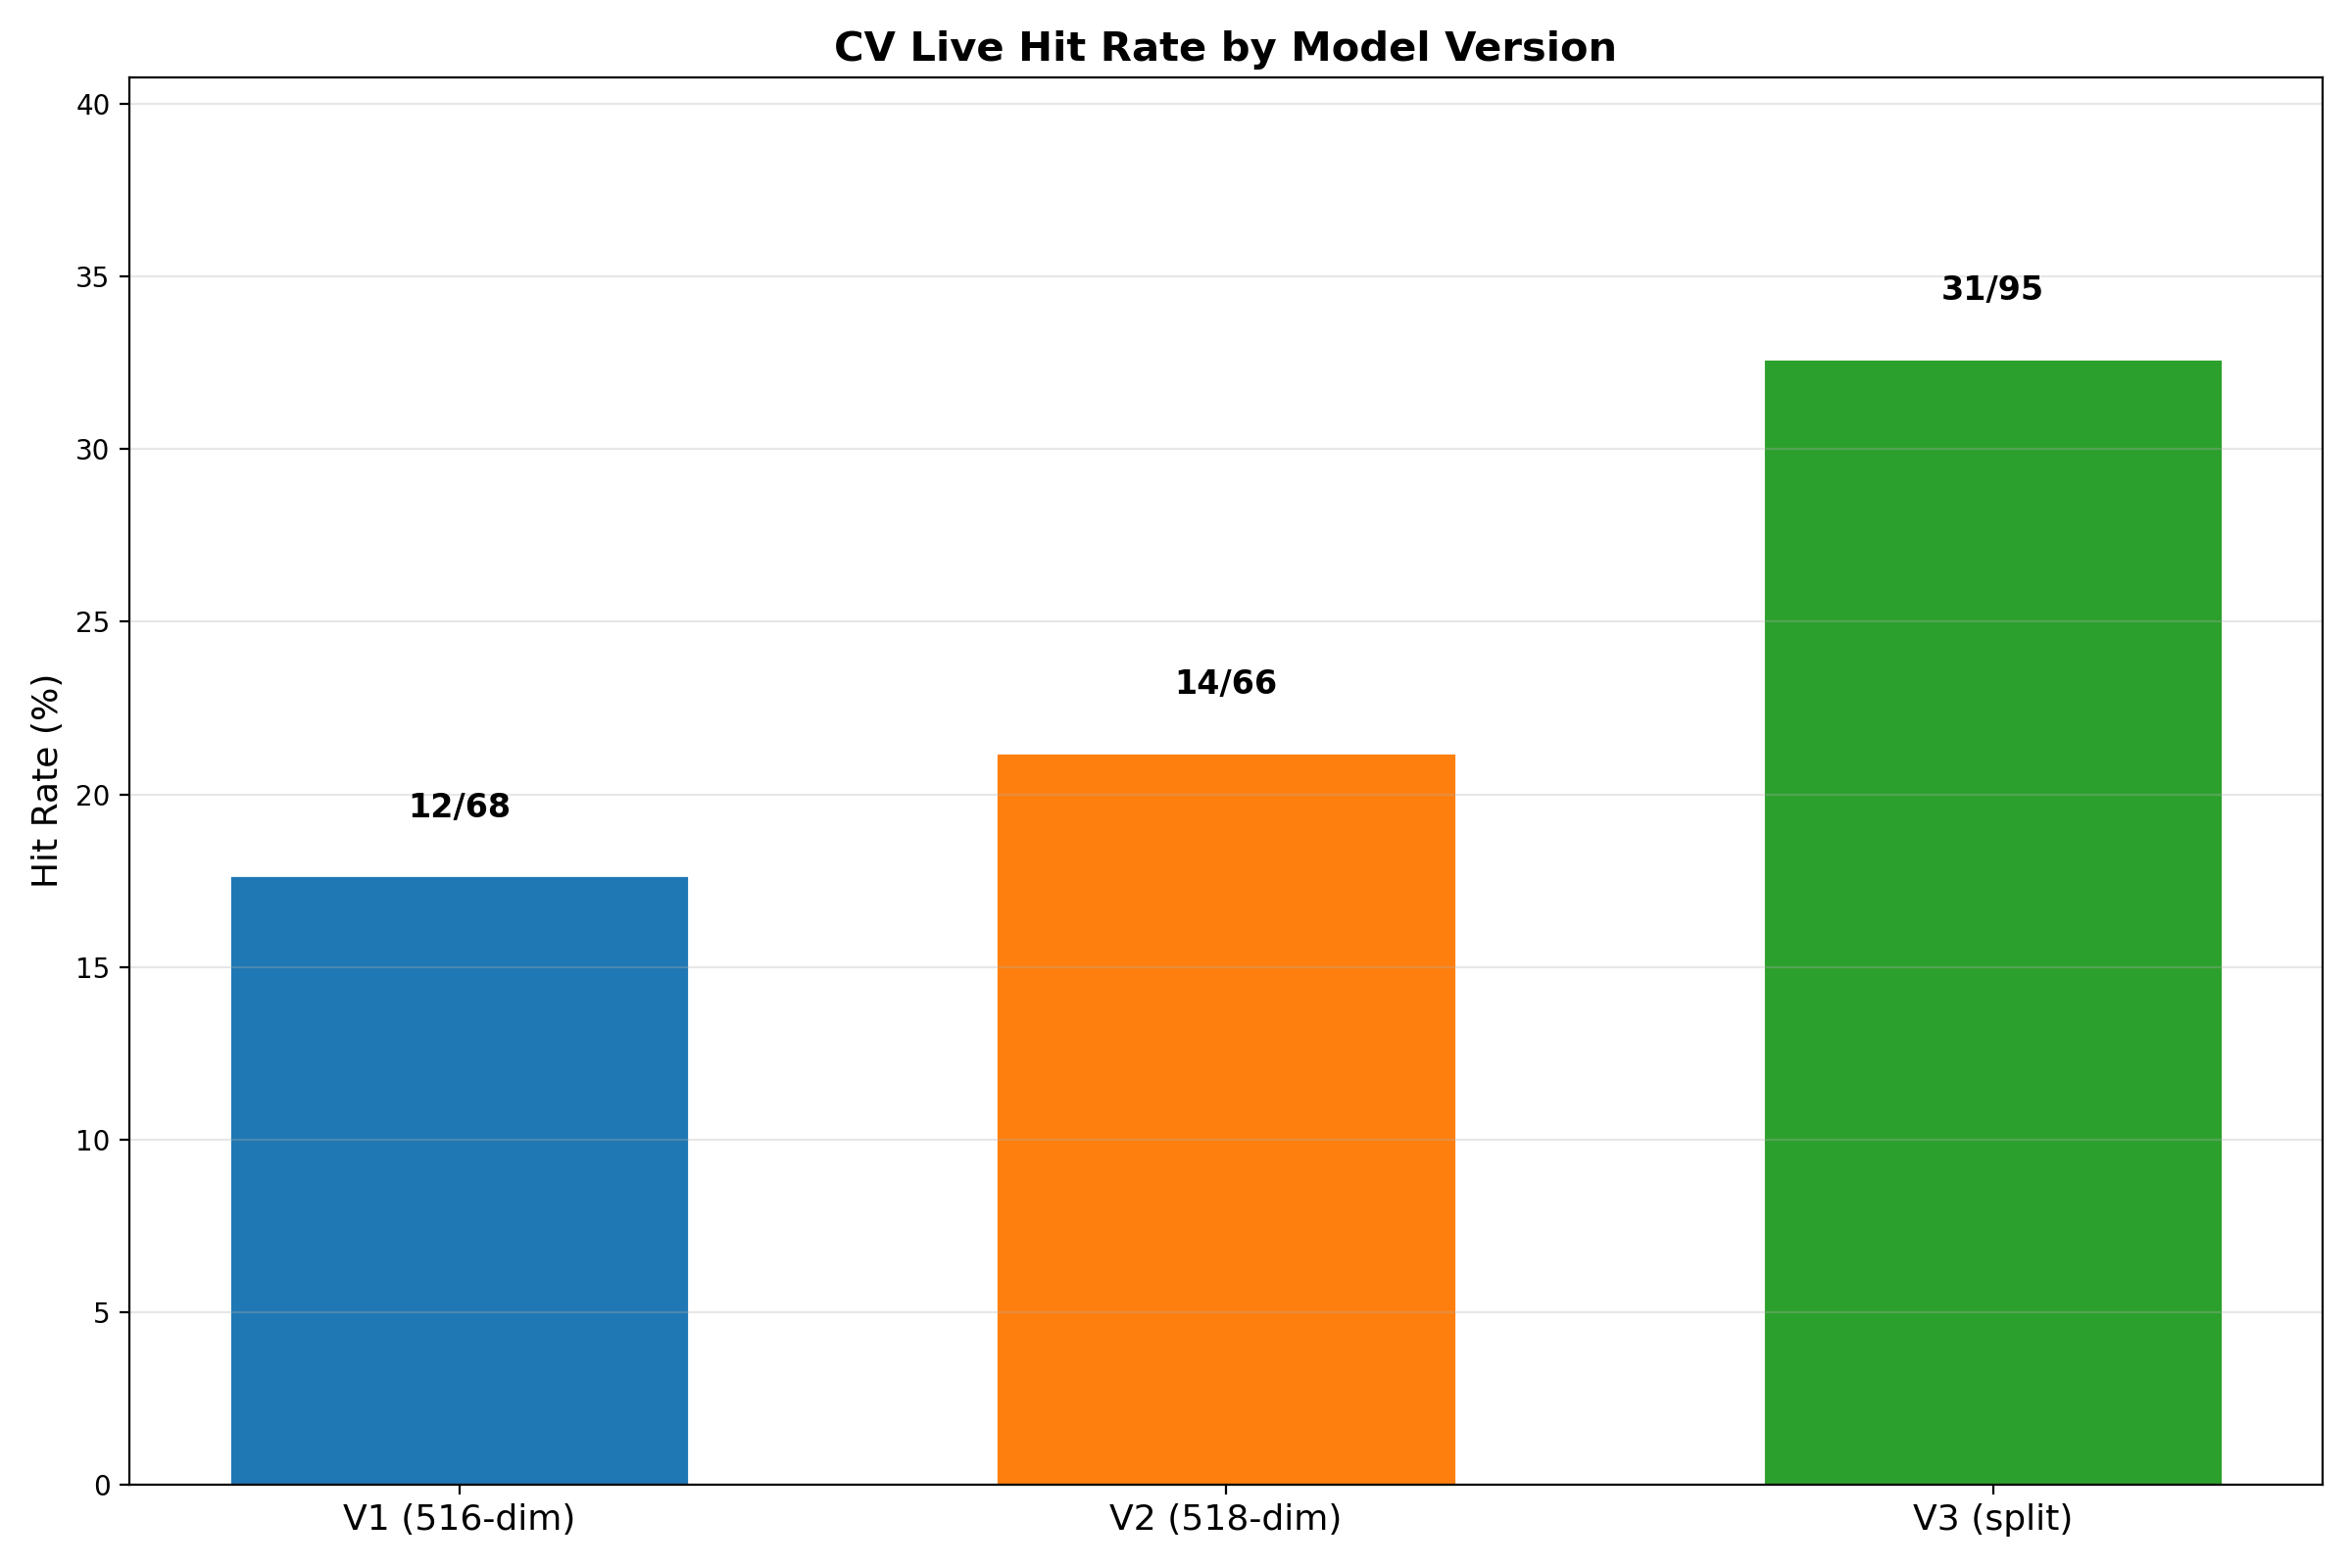
\includegraphics[width=\columnwidth]{cv_model_hit_rate.png}
  \caption{Live hit rate comparison across the three aim head model versions
  (V1: 18\%, V2: 21\%, V3: 33\%).  Hit counts and total shots are annotated
  above each bar.}
  \label{fig:hitrate}
\end{figure}

V3 achieves a 33\% live hit rate, nearly double V1's 18\%, and covers 24 of 30
distinct cup positions.  The progression from V1 to V3 validates the design
strategy: adding depth-encoding derived features in V2 improved $Y$ prediction,
and decoupling $X$ and $Y$ heads in V3 prevented $Y$-oriented features from
degrading $X$ prediction.

\begin{figure}[ht]
  \centering
  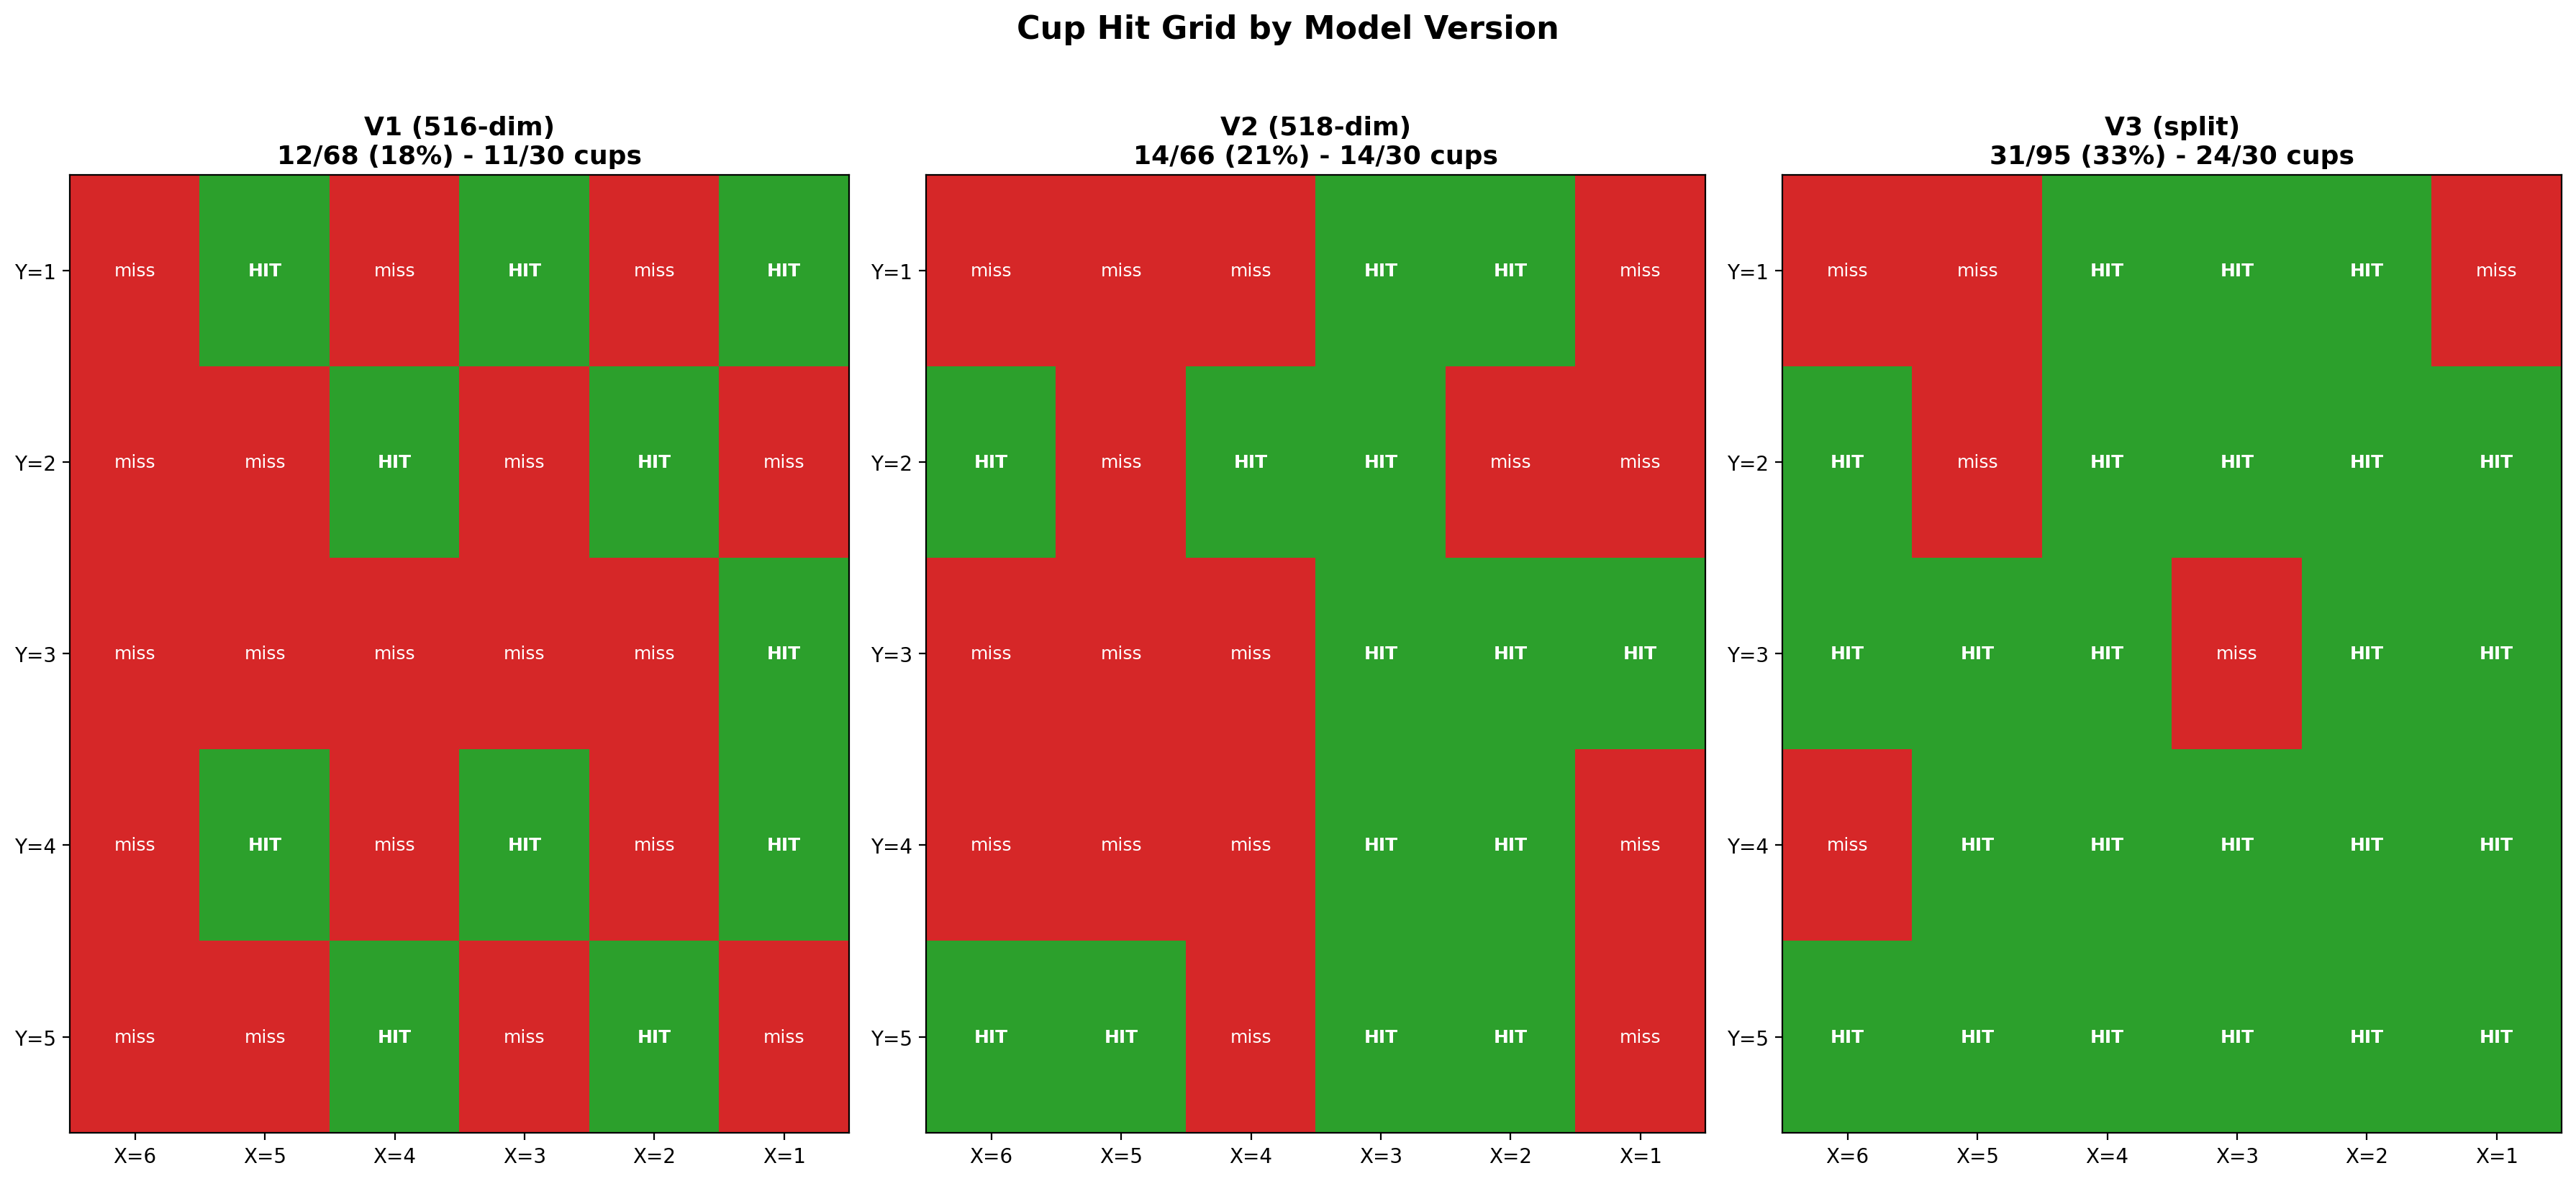
\includegraphics[width=\columnwidth]{cv_model_hit_grid.png}
  \caption{Cup hit grid ($6$ columns $\times$ $5$ rows) for each model version.
  Green $=$ hit at least once; red $=$ never hit.  V3 achieves 24/30 cups
  covered, substantially improving over V1 (11/30) and V2 (14/30), with
  improved left-side and near-row coverage.}
  \label{fig:hitgrid}
\end{figure}

The hit grid (Fig.~\ref{fig:hitgrid}) reveals that V1 and V2 struggle most with
left-side cups (columns 4-6), which are consistently missed across all rows.
V3 substantially improves left-side coverage and achieves complete near-row
coverage (rows 3-5), with the remaining weakness concentrated in the top-left
corner (columns 5-6, rows 1-2).

\subsection{Sim-to-Live Gap Analysis (4)}
\label{sec:simgap}

To compare models on a common basis, each model's predictions were evaluated
synthetically against per-cell median winning positions from RL data.  A
simulated hit requires $|X\,\text{error}| \le 400$ and
$|Y\,\text{error}| \le 400$ motor steps simultaneously.  Table~\ref{tab:gap}
and Fig.~\ref{fig:gap} report the results.

\begin{table}[ht]
\centering
\caption{Synthetic vs.\ Live Hit Rate Comparison (Sim-to-Live Gap)}
\label{tab:gap}
\setlength{\tabcolsep}{4pt}
\begin{tabular}{lrrrrrl}
\toprule
Model & MAE$_X$ & MAE$_Y$ & Bias$_X$ & Sim & Live & Gap \\
\midrule
V1 (516-dim) & 559 & 972 & $-$301 & 13\% & 18\% & $+$4\% \\
V2 (518-dim) & 439 & 657 & $-$180 & 23\% & 21\% & $-$2\% \\
V3 (split)   & 412 & 718 & $-$209 & 24\% & 33\% & $+$8\% \\
\bottomrule
\end{tabular}
\end{table}

\begin{figure}[ht]
  \centering
  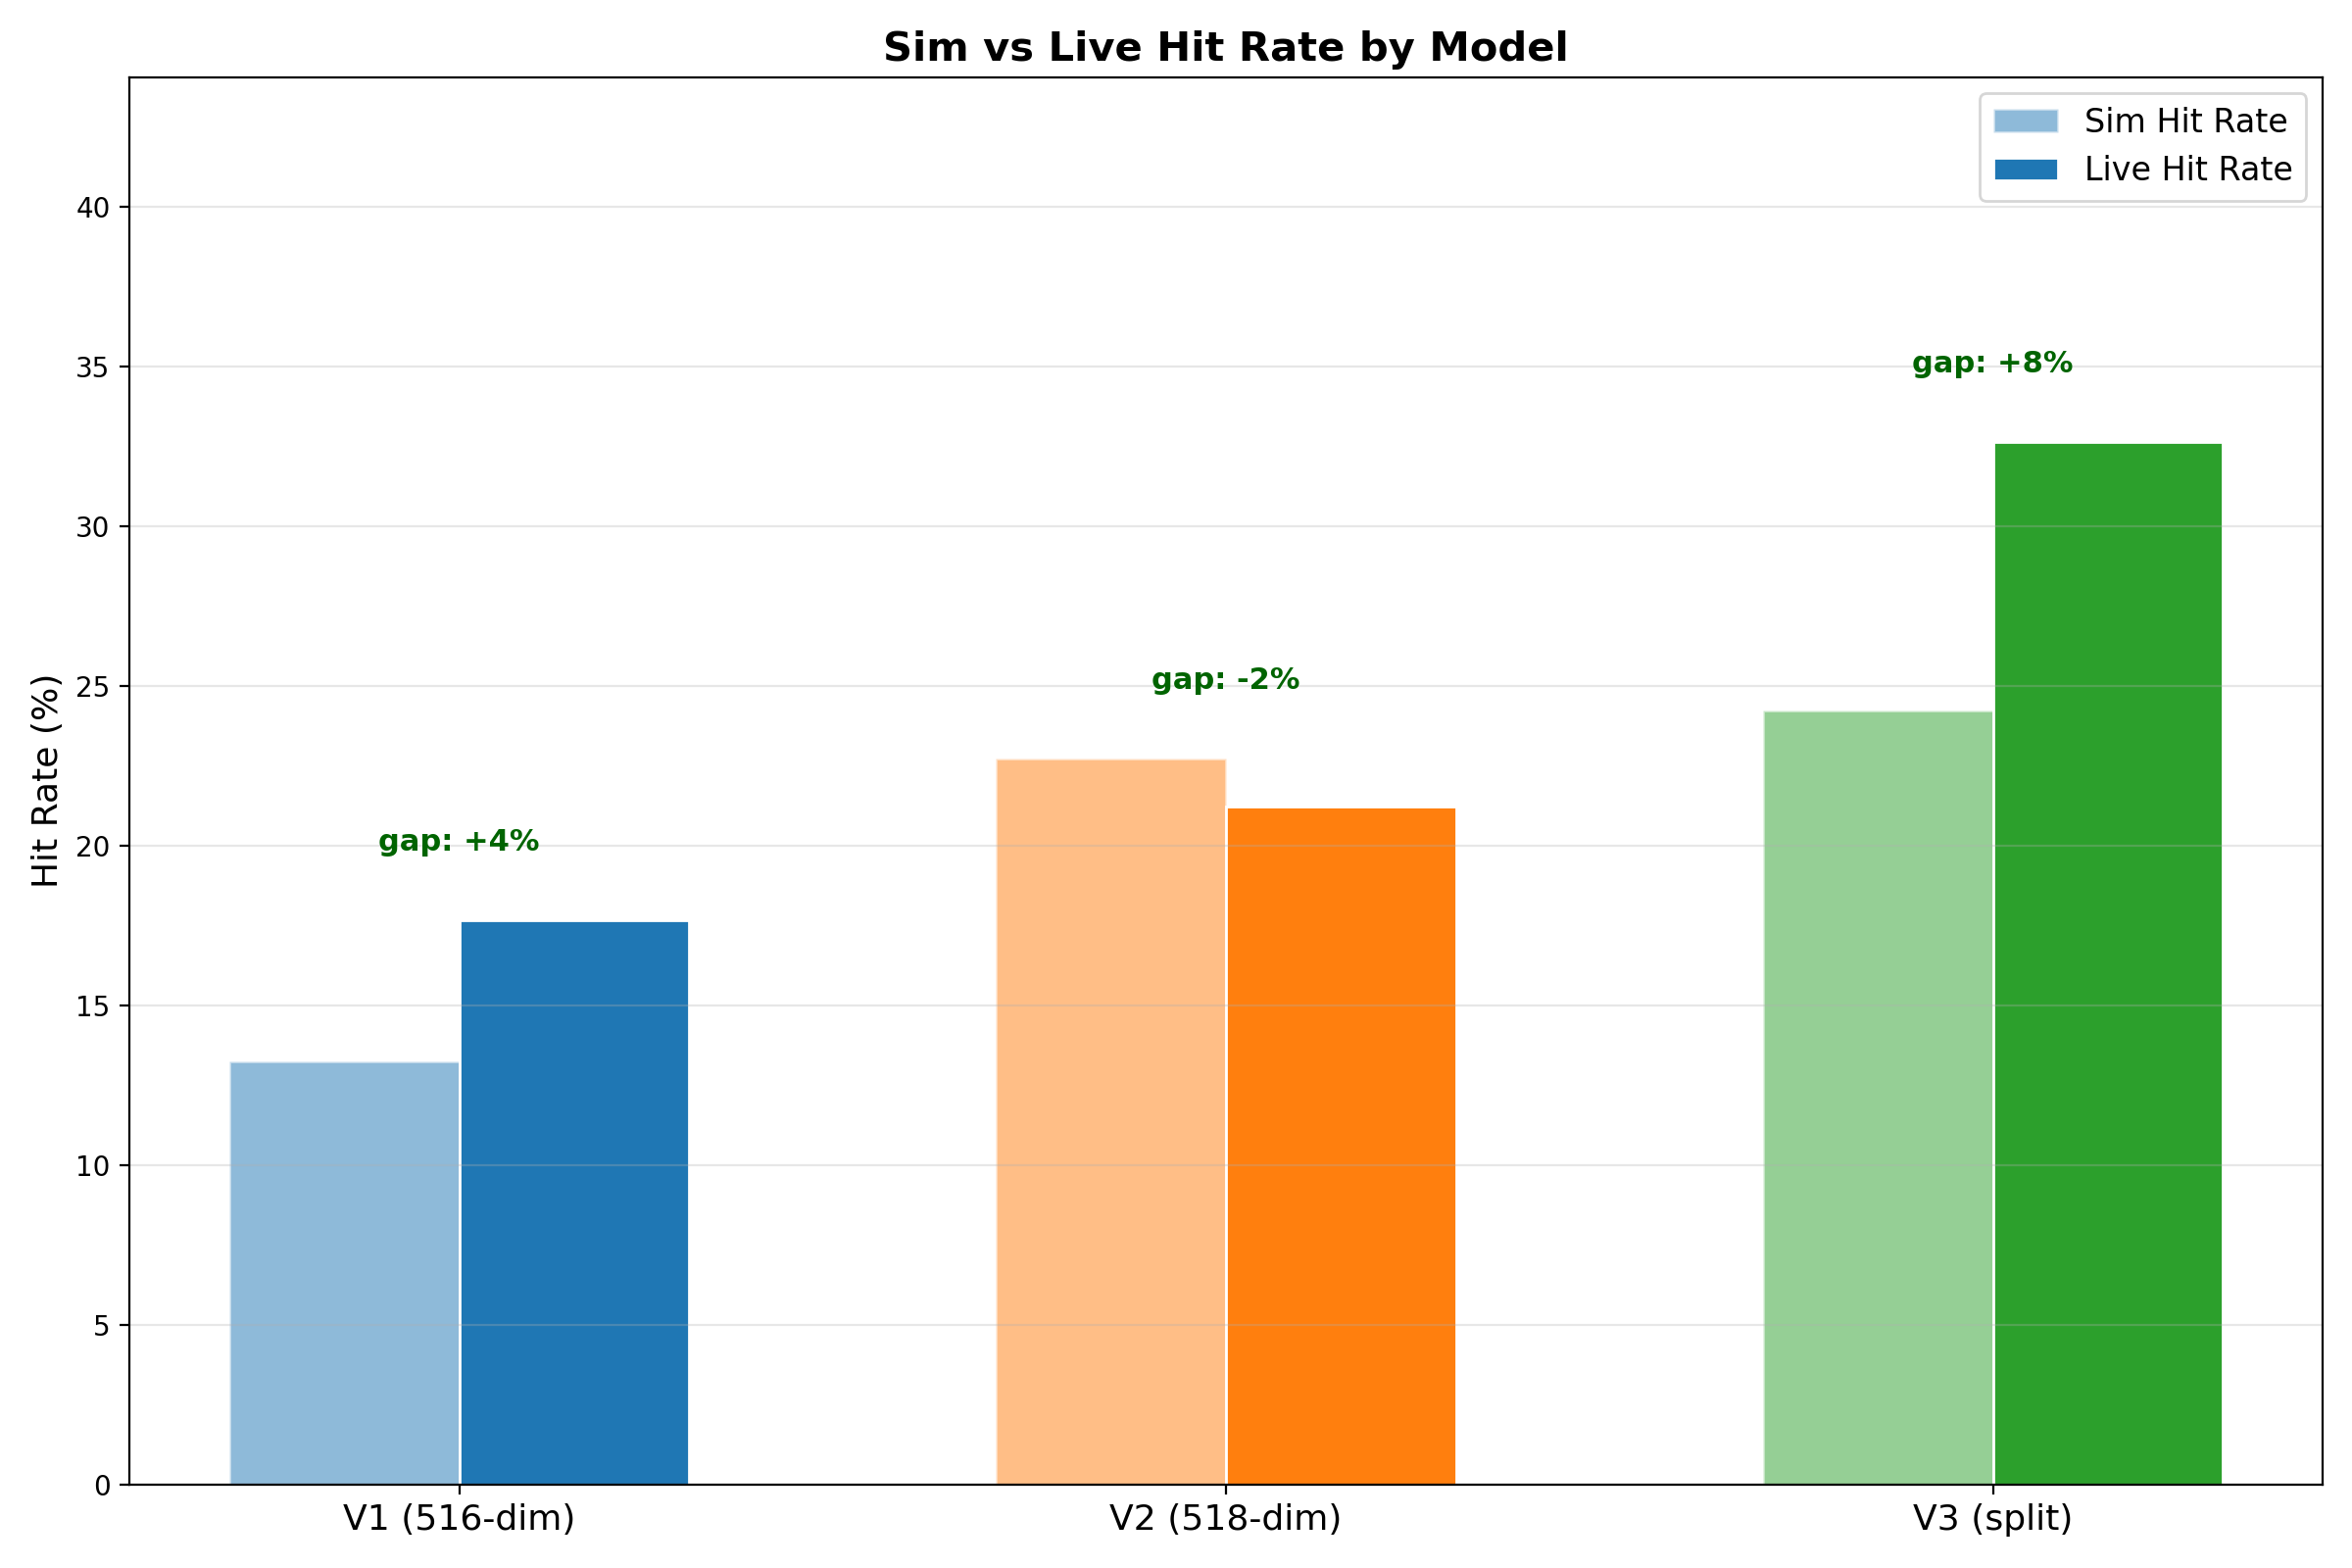
\includegraphics[width=\columnwidth]{cv_model_sim_live_gap.png}
  \caption{Sim vs.\ live hit rate per model.  Light bars represent synthetic
  (offline) hit rates; dark bars represent live hit rates.  Gap values are
  annotated.  V2 has the most calibrated predictions (gap $= -2\%$); V3's
  live rate substantially exceeds its synthetic rate (gap $= +8\%$), indicating
  predictions that are well-centred on physical targets.}
  \label{fig:gap}
\end{figure}

The sim-to-live gap is the most informative deployment metric.  V1's gap of
$+4\%$ is modest but occurs alongside a very low live rate (18\%), indicating
that its predictions are occasionally near the target but not reliably so.  V2
achieves the smallest gap ($-2\%$), meaning its synthetic and live rates are
nearly identical, its predictions are well-calibrated but not accurate enough
to yield a high hit rate (21\%).  V3 has the largest positive gap ($+8\%$),
with live rate (33\%) substantially exceeding sim rate (24\%).  This suggests
V3's predictions, while not always within the strict $\pm400$-step synthetic
threshold, are close enough to the target in practice that the ball's physical
margin of error accounts for the difference.

The consistent negative $X$ bias across all models (V1: $-301$, V2: $-180$,
V3: $-209$ steps) indicates a systematic leftward prediction offset that is not
fully corrected by the split-head design.  This is consistent with the
per-column error analysis in Table~\ref{tab:percolumn} and likely reflects a
systematic offset in launcher calibration or the camera's mounting angle
introducing a consistent positional bias across the table.  The substantially
higher MAE$_Y$ in V1 (972) compared to V2 (657) and V3 (718) quantifies the
improvement from adding depth-encoding derived features.  Despite V3's
slightly higher MAE$_Y$ than V2 (718 vs.\ 657), its live hit rate is
substantially better (33\% vs.\ 21\%), suggesting that the split-head
architecture produces predictions that are better distributed around the true
target even if the mean error is slightly larger.

% --- VI. Conclusions ---------------------------------------------------------
\section{Conclusions and Future Work}
\label{sec:conclusions}

This paper presented a complete computer vision pipeline for single-shot cup
aim prediction from a camera on a Raspberry Pi, addressing all four stated
research objectives.

\textbf{1 achieved.}  The full PongDetector and aim head (V3) were
successfully exported to ONNX and deployed on the Raspberry Pi via
\texttt{cv2.dnn} with no PyTorch dependency, running at approximately
830\,ms per inference on the ARM Cortex-A72.

\textbf{2 achieved.}  The $r^{2}$ correlation analysis (Fig.~\ref{fig:r2},
Table~\ref{tab:r2}) revealed that backbone features are position-blind
($r^{2}=0.117$ with $x$-position) while bbox $c_x$ achieves $r^{2}=0.981$,
motivating explicit bounding box concatenation as a principled architecture
decision.

\textbf{3 achieved.}  Iterative development of V1$\to$V2$\to$V3 demonstrates
progressive improvement (18\%$\to$21\%$\to$33\% live hit rate, 11/30$\to$14/30
$\to$24/30 cups covered).  The split-head design is the most effective
architecture.

\textbf{4 achieved.}  The sim-to-live gap analysis reveals that V3 achieves
the highest live hit rate (33\%) despite its larger positive gap ($+8\%$),
while V2's near-zero gap ($-2\%$) indicates well-calibrated but less accurate
predictions.  The analysis shows that synthetic hit rate alone is insufficient
for evaluating deployment readiness.

\subsection*{Lessons Learned}

Explicit geometric features substantially outperform learned backbone
representations for spatial regression; bounding box coordinates provide the
dominant signal for both axes.  The sim-to-live gap is a more reliable
deployment metric than synthetic hit rate alone, as physical tolerances can
cause live performance to diverge from offline evaluation in either direction.
Per-cell median denoising of RL pseudo-labels meaningfully reduces $Y$
prediction variance.

\subsection*{Future Work}

Five directions would further improve performance.

(1)~\textit{Improved camera geometry:} mounting the camera at a higher angle
would increase variation of cup $c_y$ across the depth range, making $c_y$ a
stronger $Y$ predictor.

(2)~\textit{Additional depth features:} exploring perspective-corrected
features or explicit focal-length-based depth estimation could provide stronger
$Y$-axis signal beyond bounding box height alone.

(3)~\textit{RT-DETR backbone}~\cite{zhao2024}: a transformer-based real-time
detector could improve detection quality and provide richer spatial features
while remaining edge-deployable.

(4)~\textit{Arbitrary cup placement:} the current system assumes cups are
placed on a fixed $6{\times}5$ grid, with pseudo-labels derived from RL
sessions targeting known positions.  Extending to arbitrary cup locations would
require a more general aim regression approach, removing the dependency on a
predefined grid for both data collection and evaluation.

(5)~\textit{Multi-cup detection:} the current system detects a single cup per
shot.  Extending to a multi-object detection backbone would enable the system
to plan a sequence of shots targeting all visible cups without requiring
repositioning between shots.

% --- References --------------------------------------------------------------
\bibliographystyle{IEEEtran}

\begin{thebibliography}{99}

\bibitem{redmon2016}
J.~Redmon, S.~Divvala, R.~Girshick, and A.~Farhadi,
``You Only Look Once: Unified, Real-Time Object Detection,''
in \textit{Proc. IEEE CVPR}, 2016, pp.~779--788.

\bibitem{he2016}
K.~He, X.~Zhang, S.~Ren, and J.~Sun,
``Deep Residual Learning for Image Recognition,''
in \textit{Proc. IEEE CVPR}, 2016, pp.~770--778.

\bibitem{hu2018}
J.~Hu, L.~Shen, and G.~Sun,
``Squeeze-and-Excitation Networks,''
in \textit{Proc. IEEE CVPR}, 2018, pp.~7132--7141.

\bibitem{lin2017}
T.~Lin, P.~Goyal, R.~Girshick, K.~He, and P.~Dollar,
``Focal Loss for Dense Object Detection,''
in \textit{Proc. IEEE ICCV}, 2017, pp.~2980--2988.

\bibitem{saxena2008}
A.~Saxena, L.~L.~S.~Wong, and A.~Y.~Ng,
``Learning Grasp Strategies with Partial Shape Information,''
in \textit{Proc. AAAI Conf. Artif. Intell.}, 2008, pp.~1491--1494.

\bibitem{lepetit2009}
V.~Lepetit, F.~Moreno-Noguer, and P.~Fua,
``EPnP: An Accurate O(n) Solution to the PnP Problem,''
\textit{Int. J. Comput. Vis.}, vol.~81, no.~2, pp.~155--166, 2009.

\bibitem{redmon2015}
J.~Redmon and A.~Angelova,
``Real-Time Grasp Detection Using Convolutional Neural Networks,''
in \textit{Proc. ICRA}, 2015, pp.~1316--1322.

\bibitem{levine2018}
S.~Levine, P.~Pastor, A.~Krizhevsky, J.~Ibarz, and D.~Quillen,
``Learning Hand-Eye Coordination for Robotic Grasping with Deep Learning and
Large-Scale Data Collection,''
\textit{Int. J. Robot. Res.}, vol.~37, no.~4--5, pp.~421--436, 2018.

\bibitem{jocher2020}
G.~Jocher et al.,
``YOLOv5 by Ultralytics,''
Zenodo, 2020. [Online]. Available: \url{https://github.com/ultralytics/yolov5}

\bibitem{jocher2023}
G.~Jocher, A.~Chaurasia, and J.~Qiu,
``YOLO by Ultralytics (Version 8.0),''
Zenodo, 2023.

\bibitem{zheng2020}
Z.~Zheng, P.~Wang, W.~Liu, J.~Li, R.~Ye, and D.~Ren,
``Distance-IoU Loss: Faster and Better Learning for Bounding Box Regression,''
in \textit{Proc. AAAI}, 2020, pp.~12993--13000.

\bibitem{zhao2024}
H.~Zhao, L.~Zhang, and H.~Hu,
``DETRs Beat YOLOs on Real-time Object Detection,''
in \textit{Proc. IEEE CVPR}, 2024.

\end{thebibliography}

\end{document}
